\documentclass[a4paper]{article}
\usepackage{hyperref}
\usepackage{graphicx}
\usepackage{listings}
\usepackage{xcolor}

\colorlet{punct}{red!60!black}
\definecolor{background}{HTML}{EEEEEE}
\definecolor{delim}{RGB}{20,105,176}
\colorlet{numb}{magenta!60!black}
\graphicspath{ {./img/} }
\lstdefinelanguage{json}{
    basicstyle=\normalfont\ttfamily,
    %numbers=left,
    numberstyle=\scriptsize,
    stepnumber=1,
    numbersep=8pt,
    showstringspaces=false,
    breaklines=true,
    frame=lines,
    backgroundcolor=\color{background},
    literate=
     *{0}{{{\color{numb}0}}}{1}
      {1}{{{\color{numb}1}}}{1}
      {2}{{{\color{numb}2}}}{1}
      {3}{{{\color{numb}3}}}{1}
      {4}{{{\color{numb}4}}}{1}
      {5}{{{\color{numb}5}}}{1}
      {6}{{{\color{numb}6}}}{1}
      {7}{{{\color{numb}7}}}{1}
      {8}{{{\color{numb}8}}}{1}
      {9}{{{\color{numb}9}}}{1}
      {:}{{{\color{punct}{:}}}}{1}
      {,}{{{\color{punct}{,}}}}{1}
      {\{}{{{\color{delim}{\{}}}}{1}
      {\}}{{{\color{delim}{\}}}}}{1}
      {[}{{{\color{delim}{[}}}}{1}
      {]}{{{\color{delim}{]}}}}{1},
}

\setlength\parindent{0pt}

\begin{document}

\section{Ambiente di lavoro}

Per prima cosa dobbiamo installare e configurare il nostro ambiente di lavoro principale. I software necessari sono piuttosto "pesanti" e quindi vi chiediamo di scaricarli da casa.

\newpage
\subsection{Software da scaricare}
Vi chiediamo di scaricare 

\begin{itemize}
    \item \LaTeX da \url{https://www.tug.org/texlive/}
    \item Anaconda (Python) da \url{https://www.anaconda.com/}
    \item Visual Studio Code da \url{https://code.visualstudio.com/}
\end{itemize}




\subsection{Configurazione Visual Studio Code e estensioni}
Installare il software di sviluppo Visual Studio Code:  \\
\url{https://code.visualstudio.com/}

Visual Studio Code ci servirà per lavorare con \LaTeX, Python e i notebook Jupyter. Dobbiamo quindi installare le estensioni per questi tre ambienti.

Per prima cosa accediamo alle estensioni si VsCode dal manu \verb|File-Preferences-Extensions|

e installiamo l'estensione Python



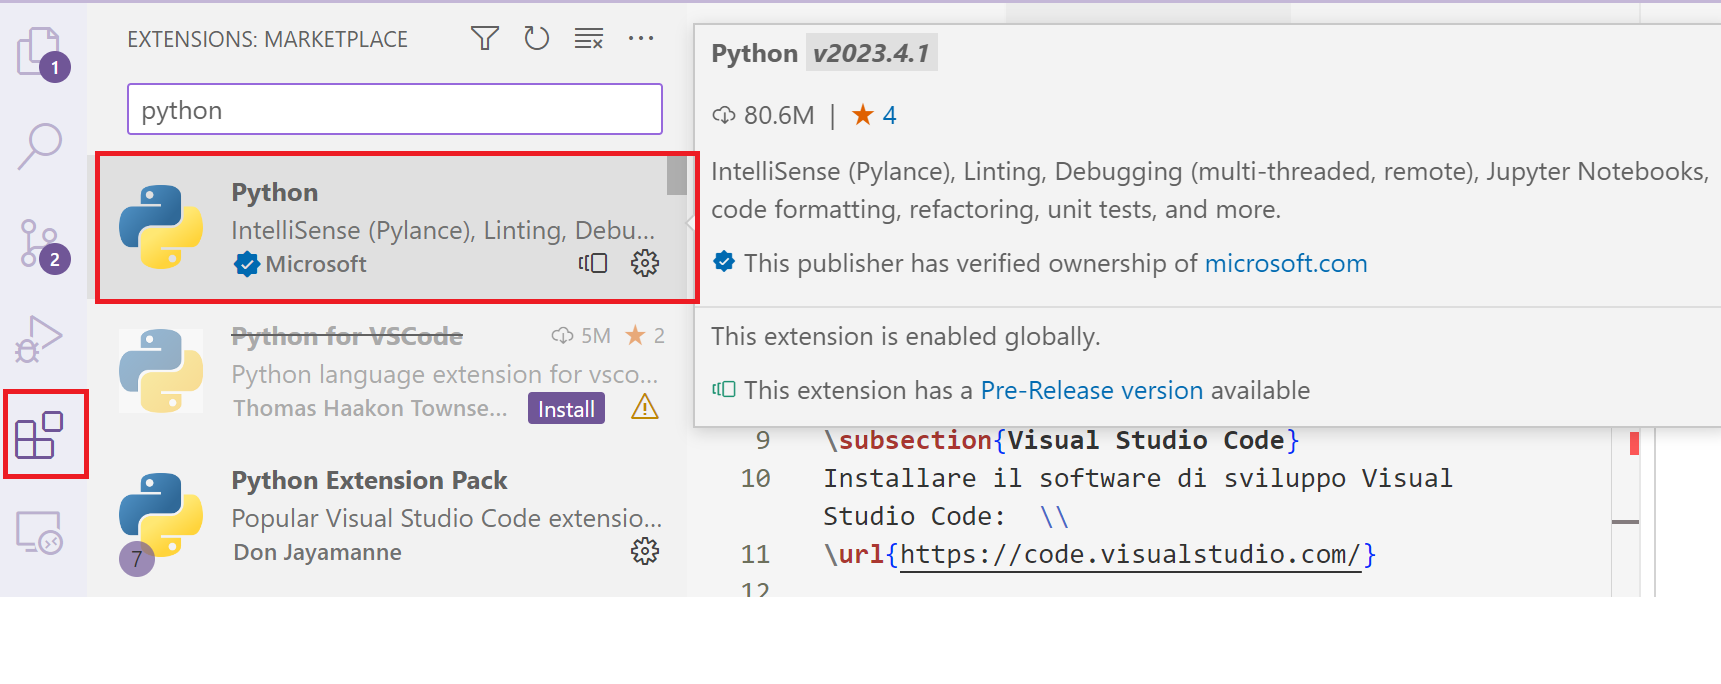
\includegraphics[scale=0.4]{vscode-python.png}

installiamo l'estensione per \LaTeX chiamata \verb|Latex Workshop|

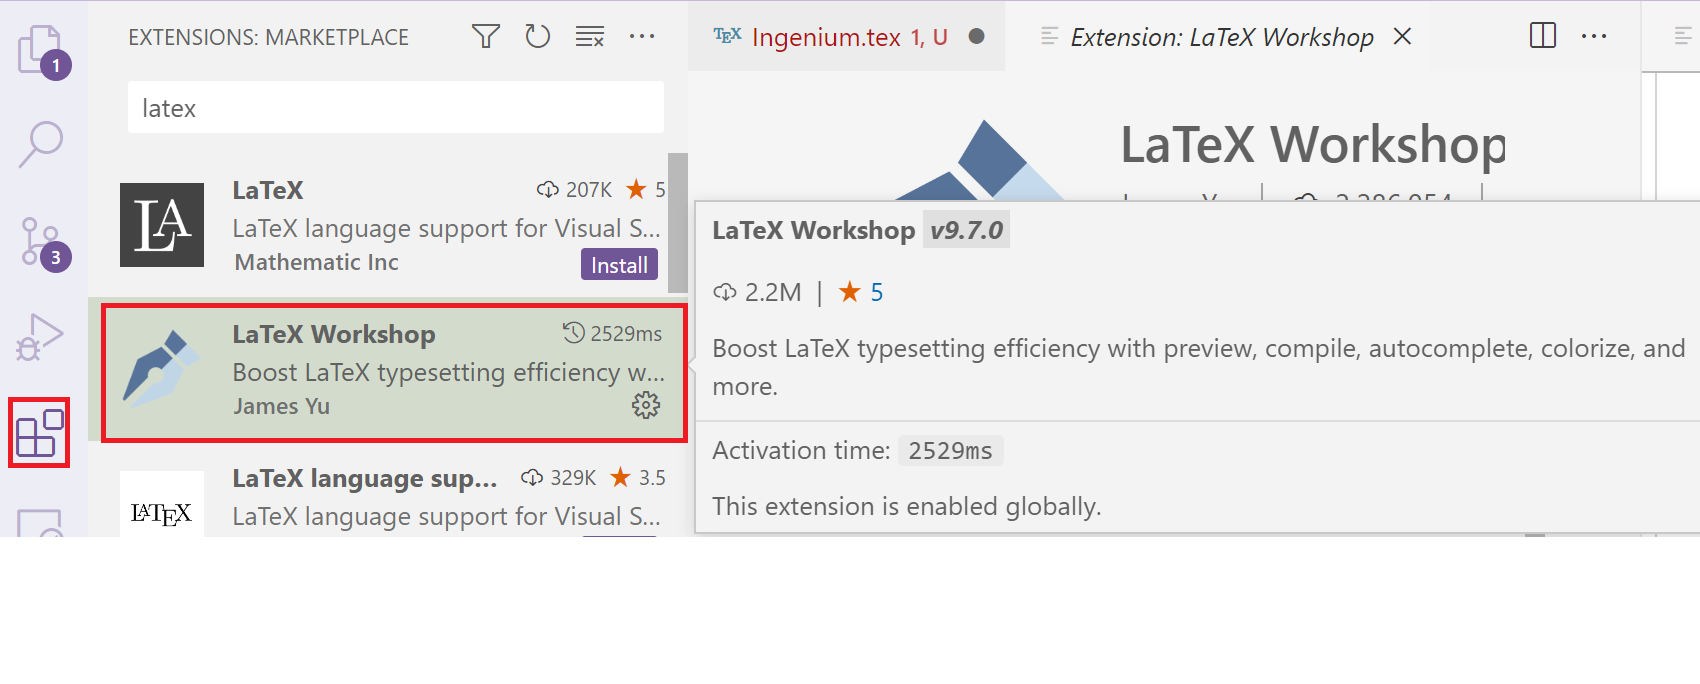
\includegraphics[scale=0.4]{vscode-latex.png}


e infine l'estensione Jupyter:

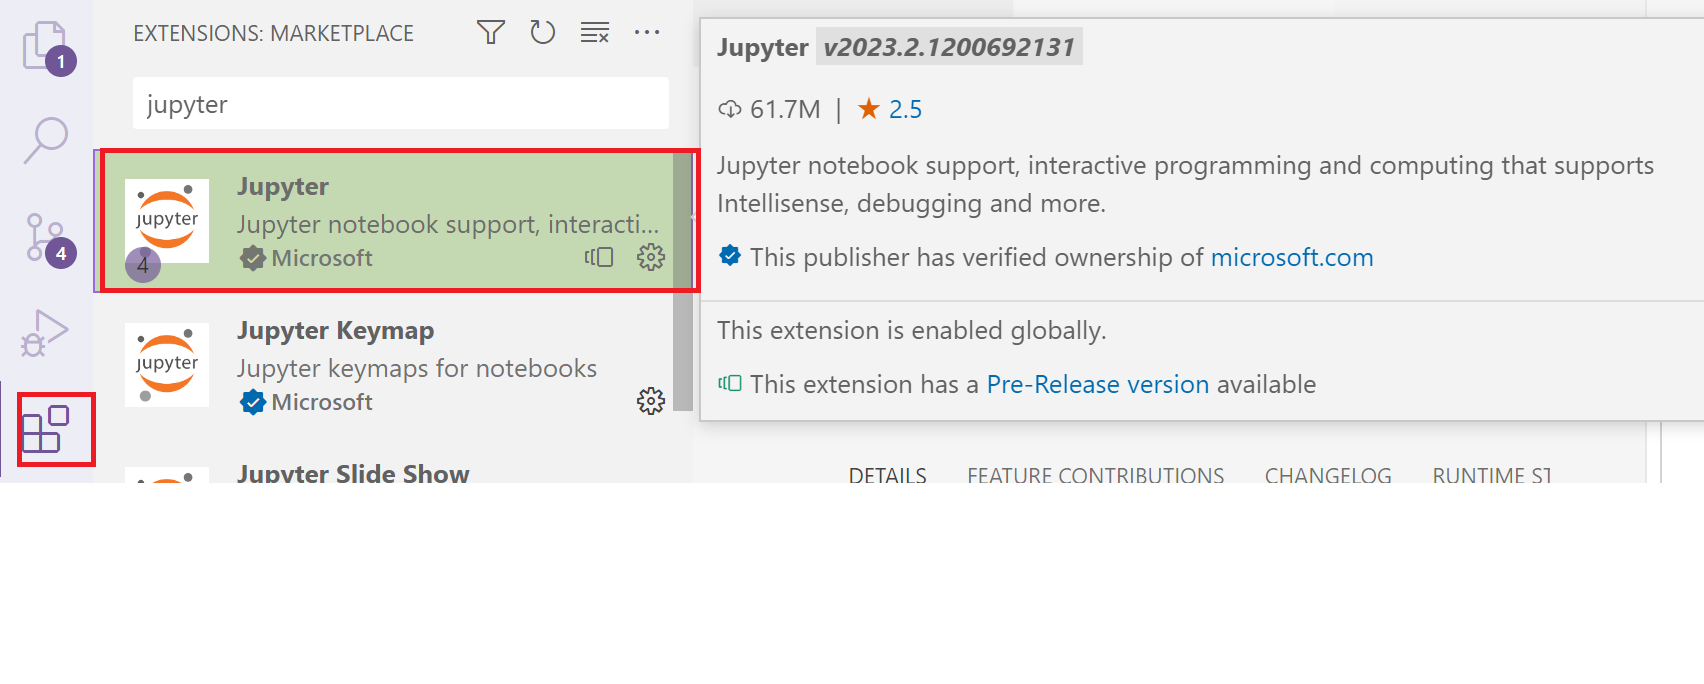
\includegraphics[scale=0.4]{img/vscode-jupyter.png}

\newpage

\subsubsection*{Configurazione estensione \LaTeX}
Per personalizzare la configurazione di \LaTeX a livello di utilizzatore aprire il file \verb|User Settings (JSON)| dalla prompt dei comandi (\verb|CTRL+SHIFT+P|)

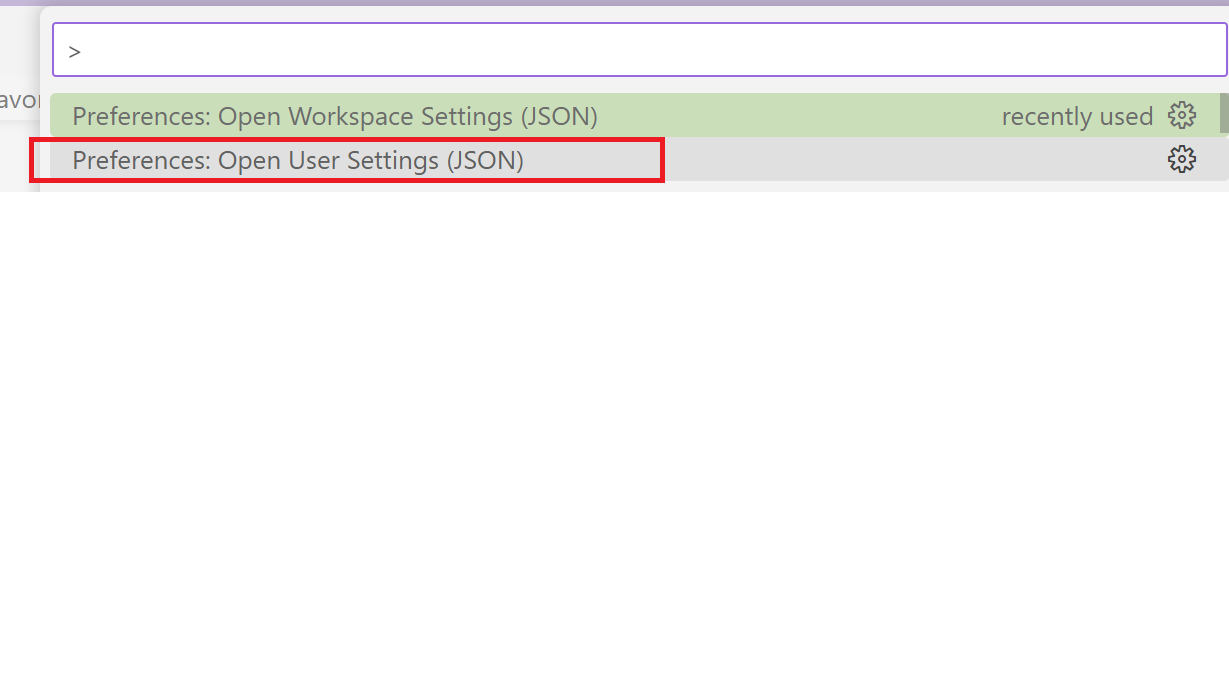
\includegraphics[scale=0.5]{img/vscode-latex-json.png}


Configurazione Windows:

\begin{lstlisting}[language=json]
    {
    "latex-workshop.latex.outDir": "%DIR%/tmp",
    "latex-workshop.latex.recipes": [
        {
          "name": "pdflatex",
          "tools": [
            "pdflatex",
            "copypdf",
          ]
        }],
        "latex-workshop.latex.tools": [
          {
            "name": "pdflatex",
            "command": "pdflatex",
            "args": [
              "-synctex=1",
              "-interaction=nonstopmode",
              "-output-directory=%OUTDIR%",
              "--shell-escape",
              "%DOC%"
            ],
            "env": {}
          },
          {
            "name": "copypdf",
            "command": "xcopy",
            "args": [
              "%OUTDIR_W32%\\%DOCFILE%.pdf",
              "%DIR_W32%\\",
              "/y"
            ]
          },
        ]
}
\end{lstlisting}


Configurazione OsX:

\begin{lstlisting}[language=json]
    {
        "latex-workshop.latex.outDir": "%DIR%/tmp",
      "latex-workshop.latex.recipes": [
          {
            "name": "pdflatex",
            "tools": [
              "pdflatex",
              "pdflatex",
              "copypdf"
            ]
          }],
          "latex-workshop.latex.tools": [
            {
              "name": "pdflatex",
              "command": "pdflatex",
              "args": [
                "-synctex=1",
                "-interaction=nonstopmode",
                "-output-directory=%OUTDIR%",
                "--shell-escape",
                "%DOC%"
              ],
              "env": {}
            },
            {
              "name": "copypdf",
              "command": "cp",
              "args": [
                "%OUTDIR_W32%/%DOCFILE%.pdf",
                "%DIR_W32%/"
              ]
            },
          ],
        
    }
\end{lstlisting}


\end{document}